\section{Zero Degree Calorimeter (ZDC) }

	Οι Zero Degree Calomieter (ZDC) ανιχνευτές αποτελούνται από τρια μέρη καλοριμέτρων. Το κάθε καλορίμετρο αποτελείται από διαδοχικά στρώματα βολφραμίου και ινών πλαστικού σπινθηριστή που παράγουν ένα οπτικό σήμα το οποίο ενισχύεται από έναν κοινό φωτοπολλαπλασιαστή, όπως φαίνεται στις Εικόνες (\ref{fig3.27}).
	
	\begin{figure}[h!]
		\centering
		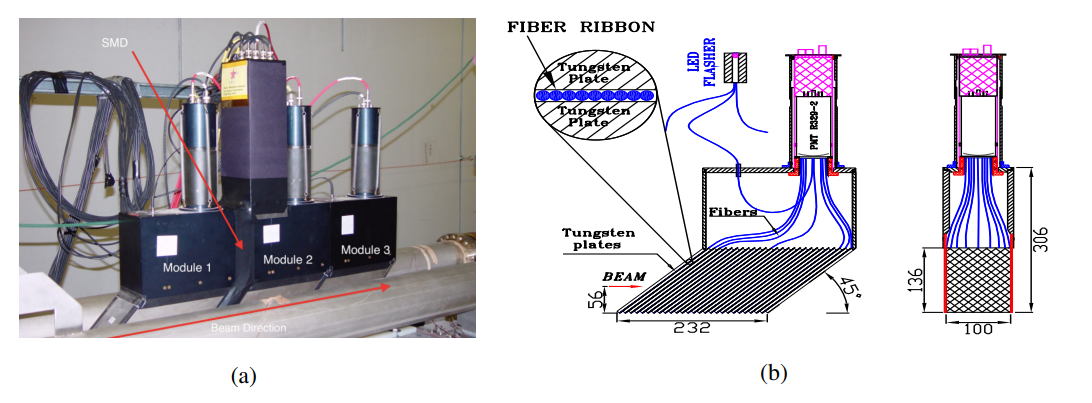
\includegraphics[scale=0.5]{STAR_Detectors/ZDC}
		\caption{Φωτογραφία του ZDC και σχέδιο του ενός από τα τρία μέρη του.}
		\label{fig3.27}
	\end{figure}
	
	Οι ZDC είναι σχεδιασμένοι για να ταυτοποιούν ουδέτερα σωματίδια και κυρίως νετρόνια που φέγουν από την περιοχή αλληλεπίδρασης σχεδόν παράλληλα με την δέσμη και ταυτόχονα παρέχουν πληροφορίες στο σύστημα \textit{trigger}. Είναι τοποθετημένοι και στις δύο πλευρές εκτός της περιοχής αλληλεπίδρασης 